\section{Diseño}
En esta sección vamos a abocarnos en la tarea de explicar el diseño que pensamos y desarrollamos para el sistema.

\subsction{Timer}

\subsection{Sensores}

\subsection{Actuadores}

\subsection{Interfaz de Usuario}

\subsection{Situación: nueva medición de humedad}
Vamos a tomar un caso para ejemplificar el comportamiento del sistema al recibir una nueva medición y su consecuente resolución.

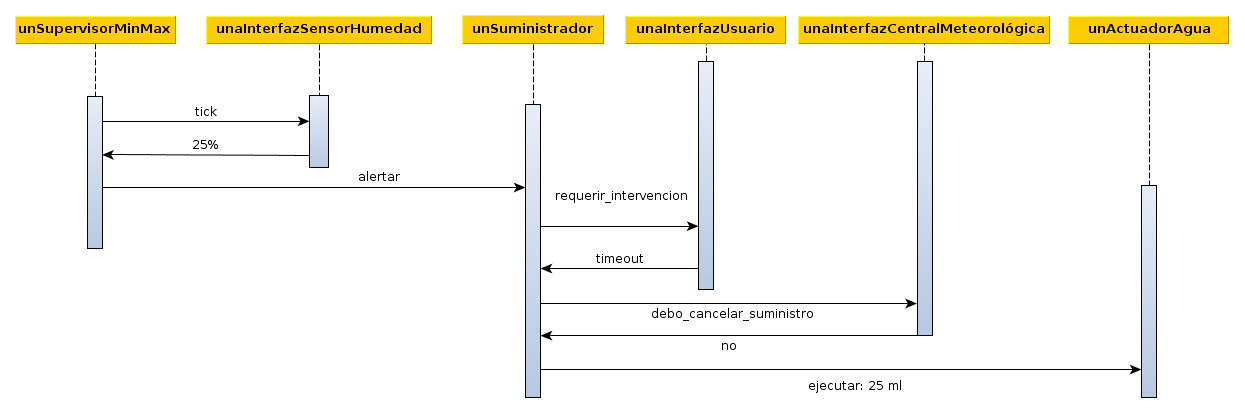
\includegraphics[width=\textwidth]{./imagenes/secuencia_alerta}

A medida que transcurre el tiempo, el temporizador envía el mensaje de actualización a los distintos supervisores. 
Los supervisores a su vez, se encargan de revisar el estado de los distintos sensores para decidir si alertar o no en caso de un estado no deseado.
En este caso, espera la respuesta de la interfaz de humedad. Como vimos antes, las interfaces de sensores cumplen el rol de responder los mensajes de pedido de actualización de estado. 
El supervisor se encarga de reconocer en los datos situaciones que deben alertarse. Es así el caso del ejemplo, donde luego de recibir la actualización alerta al suministrador correspondiente.

El suministrador, previo a ejecutar la acción para suplir la alerta, colabora con la interfaz de usuario para permitir la cancelación de la acción. En caso de no haber respuesta (timeout) consulta a un responsable secundario (en este caso, el coordinador meteorológico) que nuevamente tiene la posibilidad de cancelar la acción.

Si algún responsable responde al mensaje, (es decir, no hay timeout) el suministrador actúa según la respuesta. En caso de recibir timeout de todos los responsables, decide efectuar la acción.

La acción la realiza finalmente, el actuador correspondiente.